%%%%%%%%%%%%%%%%%%%%%%%%%%%%%%%%%%%%%%%%%%%%%%%%%%%%%%%%%%%%%%%%%%%%%%%%%%%%%%%%
%2345678901234567890123456789012345678901234567890123456789012345678901234567890
%        1         2         3         4         5         6         7         8

\documentclass[letterpaper, 10 pt, conference]{ieeeconf}  % Comment this line out if you need a4paper

%\documentclass[a4paper, 10pt, conference]{ieeeconf}      % Use this line for a4 paper

\IEEEoverridecommandlockouts                              % This command is only needed if 
% you want to use the \thanks command

\overrideIEEEmargins                                      % Needed to meet printer requirements.

%In case you encounter the following error:
%Error 1010 The PDF file may be corrupt (unable to open PDF file) OR
%Error 1000 An error occurred while parsing a contents stream. Unable to analyze the PDF file.
%This is a known problem with pdfLaTeX conversion filter. The file cannot be opened with acrobat reader
%Please use one of the alternatives below to circumvent this error by uncommenting one or the other
%\pdfobjcompresslevel=0
%\pdfminorversion=4

% See the \addtolength command later in the file to balance the column lengths
% on the last page of the document

% The following packages can be found on http:\\www.ctan.org
\usepackage{graphicx} % for pdf, bitmapped graphics files
%\usepackage{epsfig} % for postscript graphics files
%\usepackage{mathptmx} % assumes new font selection scheme installed
%\usepackage{times} % assumes new font selection scheme installed
%\usepackage{amsmath} % assumes amsmath package installed
%\usepackage{amssymb}  % assumes amsmath package installed

\usepackage{xcolor}
\usepackage{balance}
\usepackage{algorithm,algorithmic}
\usepackage{subcaption}



\title{\LARGE \bf
    ROADWHERE: A UNet model for road detection through semantic segmentation of road images
}


\author{Vijay Jaisankar, Jaya Sreevalsan Nair}

\begin{document}



\maketitle
\thispagestyle{empty}
\pagestyle{empty}


%%%%%%%%%%%%%%%%%%%%%%%%%%%%%%%%%%%%%%%%%%%%%%%%%%%%%%%%%%%%%%%%%%%%
\begin{abstract}
In this paper, we propose ROADWHERE, a UNet model for road detection. We explore dataset size reduction through difference hashing and evaluate the efficacy of pretrained CNN encoders in semantic segmentation. By using a pre-trained VGG-19 backbone, we obtain a validatoin IOU score of 70.02\% using just 12.20\% of the training data. 
\end{abstract}

\section{INTRODUCTION}
\label{intro}

\subsection{Automated Driving Systems}
\label{intro:ads}
The quality and robustness of Automated Driving Systems(ADSs) have greatly improved in the era of Deep Learning (DL). They are increasingly adopted to realise their potential benefits like preventing accidents, reducing emissions, transporting the mobility-impaired and reducing driving related stress~\cite{9046805}. 
The McKinsey Center for Future Mobility Analysis shows that autonomous driving could generate \$300 Million to \$400 Million by 2035~\cite{Deichmann_Ebel_Heineke_Heuss_Kellner_Steiner_2023}. 

\subsection{Semantic Segmentation}
\label{intro:semseg}
Semantic segmentation refers to the pixel-wise labeling of an image~\cite{doi:10.1080/08839514.2022.2032924}.
As opposed to conventional object detection, the pixel-wise fine-grained outputs of semantic segmentation models provide additional rigour to ADSs. 

\subsection{Road Detection}
\label{intro:road}
In this paper, we consider the task of \textbf{Road detection}. In particular, given an RGB image of a traffic scenario, our task is to localise the pixels containing the road surface.

\begin{figure}
\centering
\begin{subfigure}{0.20\textwidth}
    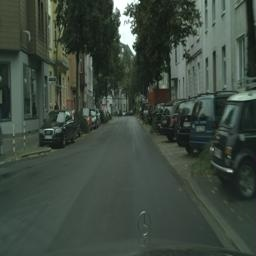
\includegraphics[width=\textwidth]{road_image_example.jpg}
    \caption{Traffic scenario}
    \label{road:image}
\end{subfigure}
\hfill
\begin{subfigure}{0.20\textwidth}
    
\includegraphics[width=\textwidth]{road_mask_example.jpg}
    \caption{Binary road mask}
    \label{road:mask}
\end{subfigure}
\hfill        
\caption{An illustration of the binary road mask for a traffic scenario.}
\label{road:detection}
\end{figure}

As shown in Figure \ref{road:detection}, our aim is to differentiate the pixels of the input image belonging to the road (shown in white) from the rest of the scenario (shown in black). This is an important basic task for autonomous vehicles attempting to navigate real-world environments.


\section{Datasets}
\label{dataset}

\subsection{Description of Candidates}
There are multiple labelled datasets for the task of Automotive Semantic Segmentation. In this work, we consider the following candidates:

\begin{itemize}
    \item CityScapes~\cite{Cordts2016Cityscapes} contains $\approx$ 3000 images for training. The original dataset consists of 30 classes, of which we limit our work to locating the pixels classified as \textit{flat:road}.
    \item KITTI-Road-Segmentation~\cite{Mahna_2021} is an aggregation of sources like the KITTI Vision Benchmark~\cite{Fritsch2013ITSC}. It contains $\approx$ 250 images for training.
\end{itemize}

\subsection{The SizeDiv Metric}
\label{sizedev:intro}
For efficient and powerful training, a candidate dataset should have sufficient number of samples and diversity across them. In this regard, we propose the following metric to assess the quality of the dataset candidate.
\subsubsection{Notation}
\begin{itemize}
    \item $N$ - the number of scenario images in the training dataset
    \item $u_{i}$ - the embedding vector for the image indexed $i$ \\ ($1 \leq i \leq N$).
\end{itemize}
\subsubsection{Methodology}
As alluded to in \ref{sizedev:intro}, our candidate dataset should have (1) adequate samples and (2) high diversity $\rightarrow$ low collective similarity between samples. To compute similarity between samples, we use a pre-trained BLIP~\cite{DBLP:journals/corr/abs-2201-12086} feature extractor, as hosted on LAVIS~\cite{li-etal-2023-lavis}. For an image indexed $i$, BLIP produces $u_i$, a 768-dimensional vector, which can be compared with other images' vectors for similarity. \\
For a given dataset with $N$ images in its training dataset, we define $SizeDiv(N)$ as \\
\[ SizeDiv(N) = N \cdot \frac{{N \choose 2}}{\sum_{i=1}^{i=N-1} 
\sum_{j=i+1}^{j=N} u_i \cdot u_j} \]

Which equates to $N$ scaled to the inverse of a joint similarity score of the images as computed through their embeddings.

\begin{table}[!h]
\vspace{-2mm}
\caption{SizeDiv scores of candidate datasets}
\vspace{-4mm}
\label{sizediv:metrics}
\begin{center}
\begin{tabular}{|c|c|c|}
\hline
\textbf{Dataset name} & \textbf{N} & \textbf{SizeDiv score ($x 10^{6}$)} \\
\hline
CityScapes & 2975 & \textbf{0.676} \\
\hline
KITTI-Road-Segmentation & 250 & 0.060 \\
\hline
\end{tabular}
\end{center}
\vspace{-6mm}
\end{table}

Based on our results summarised in Table \ref{sizediv:metrics}, we note that CityScapes not only provides more data points but is also more diverse, hence leading to a better SizeDiv score.
Hence, we perform our experiments on the CityScapes dataset.
 
\section{Training set: Size reduction}
\label{hashing}

As shown in \ref{sizediv:metrics}, the Cityscapes dataset has vast diversity within its images. As we are working with a sub-problem of the original 30-class semantic segmentation task, we hypothesise that we can achieve decent results using a \textit{subset} of the allocated training set. In this regard, we explore the possibility of the \textit{Difference Hashing} algorithm as a technique to remove duplicates, resulting in a minimal and diverse dataset for training. \\ \\
Hamming distance is used as a proxy for the \textit{distance} between images. Two hashes with a Hamming distance of zero implies that the two hashes are identical (since there are no differing bits) and that the two images are identical/perceptually similar as well~\cite{Rosebrock_2021}. We use the maximum hamming distance between images as a fast threshold to remove duplicates.

\begin{table}[!h]
\vspace{-2mm}
\caption{Reduced dataset size after Difference Hashing}
\vspace{-4mm}
\label{dhash:metrics}
\begin{center}
\begin{tabular}{|c|c|c|}
\hline
\textbf{Maximum Hamming Distance} & \textbf{\#Images in reduced training dataset}  \\
\hline
10 & 2852  \\
\hline
15 & 1762 \\
\hline
20 & 363 \\
\hline
25 & 51 \\
\hline 
30 & 10 \\
\hline
\end{tabular}
\end{center}
\vspace{-6mm}
\end{table}


\section{UNet}
\label{unet}

\begin{figure}[thpb]
    \centering
    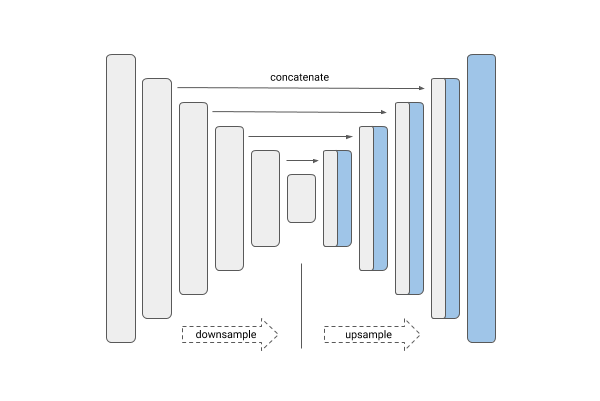
\includegraphics[scale=0.375]{unet_architecture.png}
    \caption{An overview of the UNet Architecture.}
    \label{unet:arch}
    \vspace{-4mm}
\end{figure} 

The UNet~\cite{10.1007/978-3-319-24574-4_28} is one of the most legendary architectures in the field of semantic segmentation. As shown in Figure \ref{unet:arch}, the UNet consists of two symmetrical blocks - the \textit{Encoder} and the \textit{Decoder}. 
\\
The encoder successively down-samples the images through Convolutional layers into a \textit{bottleneck} vector, which is then successively up-sampled by the decoder. \\
Crucially, \textit{skip connections} between the symmetrical stages of the encoder and decoder ensure that the model learns a mixture of low-level features and high-level features. In UNet, these features are concatenated. In LinkNet~\cite{8305148}, a variant of the UNet architecture, these features are added. \\ 

Building on the merits of transfer learning, pre-trained Convolutional Neural Networks (CNNs) are often used as backbones for the Encoder blocks. For our use-case, we make use of their immense representative power and utilise CNNs trained on Imagenet~\cite{5206848} as the encoders.

\section{Building on representations}
\label{encoder}

\subsubsection{Choosing an Encoder}
\label{encoder:preliminary}
We employ the following models as candidates for encoders through preliminary experiments:
\begin{itemize}
    \item \textit{resnet-18} from the ResNet family of models~\cite{he2016residual} was chosen due to its smaller footprint.
    \item \textit{inception-v3} from the Inception family of models~\cite{DBLP:journals/corr/SzegedyVISW15} was chosen due its deep architecture in lieu of number of layers.
    \item \textit{vgg-19} from the VGG family of the models~\cite{Simonyan15} was chosen due to its large depth and number of parameters.
\end{itemize}

To reduce the overall training time, we keep the encoders' weights frozen and split the training section of Cityscapes into a \textit{Train} section for this experiment (80\%) and \textit{Validation} section for this experiment (20\%). 

\begin{table}[!h]
\vspace{-2mm}
\caption{Training and Validation IOU Scores for the Encoder Selection Experiment}
\vspace{-4mm}
\label{encoder:metrics}
\begin{center}
\begin{tabular}{|c|c|c|c|}
\hline
\textbf{Architecture} & \textbf{Encoder} & \textbf{Train IOU} & \textbf{Val IOU}  \\
\hline
UNet & resnet-18 &  53.1772 & 52.9185 \\
\hline
UNet & inception-v3 & 53.2342 & 52.9186 \\
\hline
UNet & vgg-19 & \textbf{56.1889} & \textbf{53.9431} \\
\hline
LinkNet & resnet-18 & 53.0129 & 52.9185 \\
\hline 
LinkNet & inception-v3 & 53.4080 & 52.9186 \\
\hline
\end{tabular}
\end{center}
\vspace{-6mm}
\end{table}

Through the results summarised in Table \ref{encoder:metrics}, we choose the vanilla \textit{UNet} architecture with \textit{vgg-19} as the backbone.

\subsubsection{ROADWHERE}
\label{encoder:roadwhere}

With this background information, we set the layers of the vgg-19 encoder to trainable and run the model with the Adam optimiser~\cite{kingma:adam} for 200 epochs. 
\\
We also apply the following augmentations to the training data at random:
\begin{itemize}
    \item Changing the brightness of the images ($75\%$ original brightness $\leq$ augmented brightness $\leq$ $125\%$ original brightness)
    \item Changing the contrast of the images ($75\%$ original contrast value $\leq$ augmented contrast value $\leq$ $125\%$ original contrast value)
\end{itemize}

Our proposed solution, \textit{ROADWHERE}, was trained on the reduced Cityscapes dataset filtered with a maximum hamming distance of 20 (see Table \ref{dhash:metrics}). The validation dataset for this experiment is the entire Validation section of the Cityscapes dataset. 

Over the course of its training loop, it achieved the following IOU scores: 
\begin{table}[!h]
\vspace{-2mm}
\caption{Training and Validation IOU Scores of ROADWHERE}
\vspace{-4mm}
\label{roadwhere:metrics}
\begin{center}
\begin{tabular}{|c|c|}
\hline
\textbf{Metric} & \textbf{Value}  \\
\hline
Training IOU Score & 75.2172  \\
\hline
Validation IOU Score & 70.0203 \\
\hline
\end{tabular}
\end{center}
\vspace{-6mm}
\end{table}


\section{Discussions}
\label{discussions}

\subsection{Synthetic Data Generation}
\label{discussion:syndata}

Recent advances in diffusion and energy-based models have led to a boom in iterative image editing model pipelines like DDPM Inversion~\cite{HubermanSpiegelglas2023}. We hypothesise that the results of the "stricter" settings for Difference Hashing (i.e., higher values of the maximum hamming distance threshold) are good candidates for adding artefacts in order to generate synthetic traffic scenarios. \\ 
In this regard, we run the Difference Hashing experiment on the Validation section of the Cityscapes dataset setting the threshold to 30. \\
We make use of the publicly-available Gradio space of the LEDITS project~\cite{tsaban2023ledits} to attempt to generate the following artefacts:
\begin{itemize}
    \item Potholes - this was chosen as a representative for physical objects
    \item Rain - this was chosen as a representative for simulating adversarial weather conditions
    \item Pedestrians
\end{itemize}


\begin{figure}
\centering
\begin{subfigure}{0.20\textwidth}
    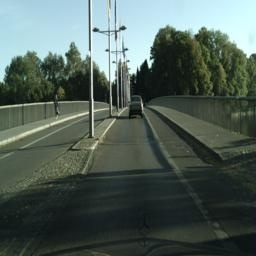
\includegraphics[width=\textwidth]{base_road_image.jpg}
    \caption{Base image given to the LEDITS model}
    \label{ledits:base}
\end{subfigure}
\hfill
\begin{subfigure}{0.20\textwidth}
    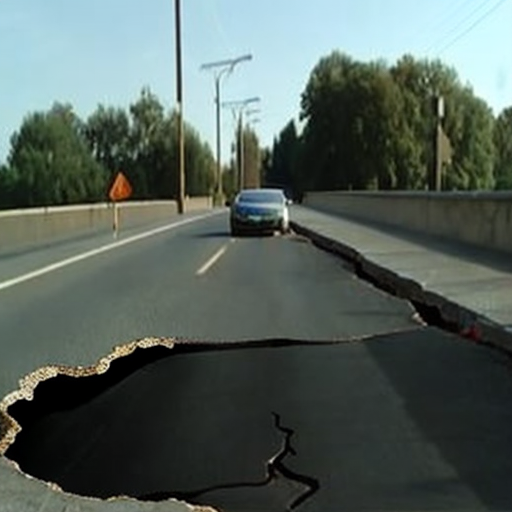
\includegraphics[width=\textwidth]{pothole_addition.png}
    \caption{LEDITS' addition of a pothole}
    \label{ledits:pothole}
\end{subfigure}
\hfill        
\begin{subfigure}{0.20\textwidth}
    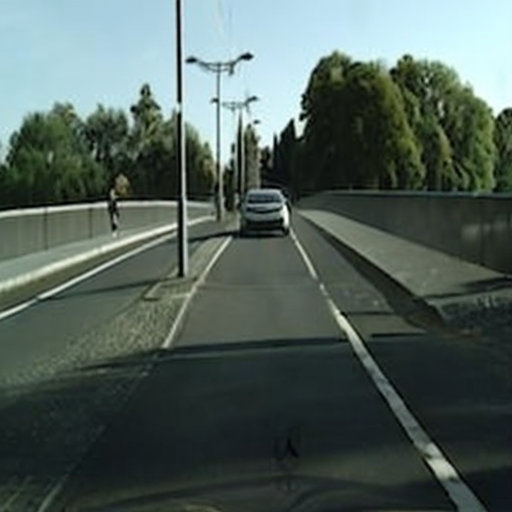
\includegraphics[width=\textwidth]{pedestrian_addition.png}
    \caption{LEDITS' addition of a pedestrian}
    \label{ledits:pedestrian}
\end{subfigure}
\hfill
\begin{subfigure}{0.20\textwidth}
    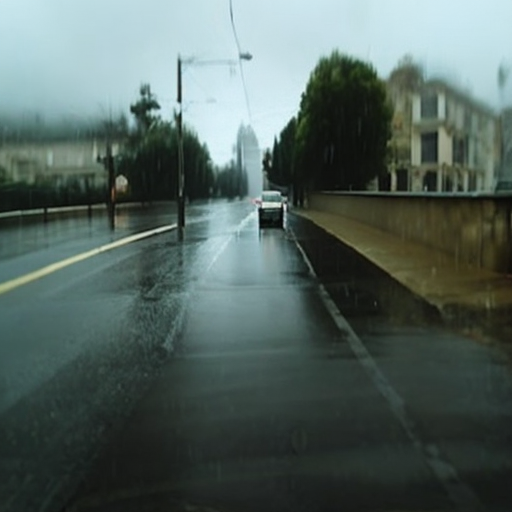
\includegraphics[width=\textwidth]{rain_addition.png}
    \caption{LEDITS' addition of rain to the scene}
    \label{ledits:rain}
\end{subfigure}
\hfill        
\caption{Qualitative results of the synthetic data generation experiment.}
\label{ledits:experiment}
\end{figure}

Qualitative results of this experiment are shown in Figure \ref{ledits:experiment}. We can see significant hallucination through addition of additional artefacts of the model in Figure \ref{ledits:rain}, wherein the trees on the right side of the frame has been replaced by a building. We also note that the content guidance factor must be increased to avoid cases like that of Figure \ref{ledits:pedestrian} wherein the desired artefacts are not added to the image at all. From our experiments, we conclude that addition of relative smaller physical objects like potholes and traffic cones is most feasible for this approach.

\subsection{Future Work}
\label{discussion:future}
We note the following themes for future work for ROADWHERE.
\begin{itemize}
    \item Experimenting with different semantic segmentation architectures like Lightweight CNN backbone-based, Multibranch backbone-based, and Transformer-based archirectures~\cite{Cheng2023}.
    \item Adversarial training and evaluating the robustness of ROADWHERE in the face of adversarial attacks like ~\cite{9956276}.
\end{itemize}


\section{Conclusion}
\label{conclusion}
In this paper, we have looked at the formulation of ROADWHERE, a VGG-19 UNet model for detecting road pixels in an image through semantic segmentation. We have also looked at the benefits of effective dataset size reduction through the results obtained. We also note some interesting future directions for this project.

\section{Acknowledgement}
\label{ack}
We would like to acknowledge the following Github repositories for their valuable implementations of crucial sections of ROADWHERE:
\begin{itemize}
    \item https://github.com/qubvel/segmentation\_models
    \item https://github.com/idealo/imagededup
    \item https://github.com/salesforce/LAVIS
    \item https://github.com/camenduru/ledits-hf
\end{itemize}

\balance
\bibliographystyle{IEEEtran}

\bibliography{references}

\end{document}